
% IDEA1: We can also make evaluation on queries where correct predicate was never seen during training. Hopefully this will show that for such queries existing approach give worse result and we somehow improve it.

% IDEA2: Hypothesis: it's easier to find mentions of the named entities rather than more abstract ones, like profession.
% Therefore, maybe errors of our model will be more on these cases?

\begin{table}
\centering
\caption{Results of experiments on combining Text2KB and STAGG predictions}
\label{table:combine_stagg}
\begin{tabular}{| p{4cm} | p{1cm} | p{1cm} | p{1cm} | }
\hline
System & avg Recall & avg Precision & avg F1 \\
\hline
Accu (baseline) \cite{ACCU:2015} & 0.604 & 0.498 & 0.494\\
% DIDN'T HAVE TIME TO IMPLEMENT THIS.
% Text-only baseline & & & & \\
Our system: Text2KB & 0.6354 & 0.5059 & 0.5223 \\
STAGG \cite{yih2015semantic} & 0.607 & 0.528 & 0.525\\
\hline
Text2KB + STAGG & 0.5976 & 0.5343 & 0.5320 \\
Text2KB + STAGG (oracle) & 0.7144 & 0.5904 & 0.6056 \\
\hline
\end{tabular}
\end{table}

In this work we took an existing KBQA systems and demonstrated that by combining evidence from knowledge base and external text resources we can boost the performance.
A reasonable question is whether the same approach will be helpful to other systems, \eg for example, can the result of the currently best system STAGG \cite{yih2015semantic} be improved.
The differences between our baseline system Accu and STAGG lie in the components, \ie entity linking algorithm, a set of query templates and ranking methods, therefore our approach is complementary and should be helpful.
To support this claim, we made an experiment to combine answers of STAGG and Text2KB.
One of the advantages of the former is its set of filters, that restricts list results to entities of certain type, gender, etc.
Therefore, we combined answers of STAGG and Text2KB using a simple heuristic: we chose to use the answer returned by STAGG if the number of answer entities is less than in the Text2KB answer, otherwise we use the answer of our approach.
Table \ref{table:combine_stagg} gives the results of the experiment, and as we can see the combination achieves slightly better average F1 score.
Alternatively, we can look at the oracle combination of the systems, which always chooses an answer with higher F1.
This experiment also verifies if both systems make the same mistakes, or there is a reasonable difference, and as we can see such a combination results in a performance of 0.6056, which is much higher than either of the systems.

WebQuestions dataset is rather small compared to the space of all possible KB queries a system should be able to generate and score.
As a result, answers to 112 of the test questions involve a predicate that weren't observed in the training set.
We also evaluated both approaches on 112 questions, where the correct answer is retrieved via a predicate, that weren't used in the positive training examples.
These questions are harder to answer, and the average F1 score of Text2KB is 0.1640 versus 0.1199 for STAGG.
This gives some anecdotal evidence, that by incorporating external text resources we were able to answer these questions slightly better, how these difference isn't statistically significant according to paired t-test (p-value 0.16).

\subsection{Error analysis}

\begin{figure}
\centering
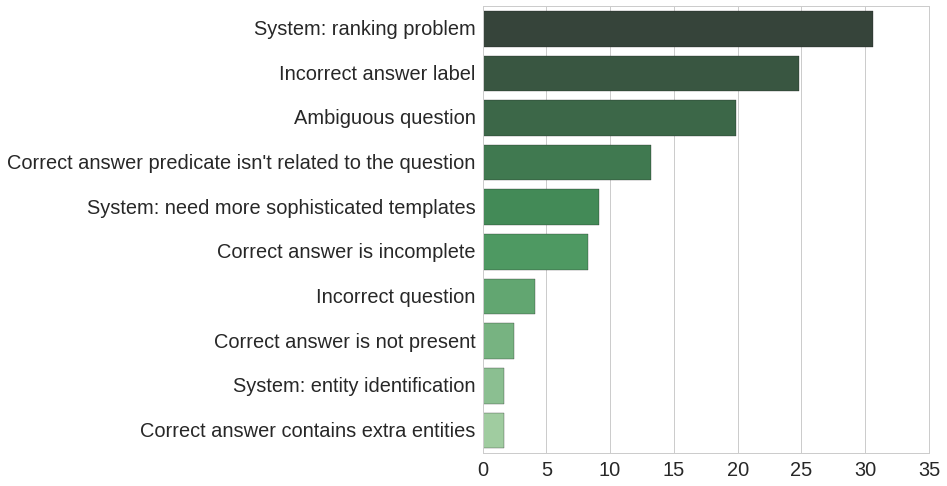
\includegraphics[width=0.45\textwidth]{img/error_analysis}
\caption{Distribution of problems with examples, where Text2KB returns an answer with F1$\neq$1.0}
\label{fig:error_analysis}
\end{figure}

To get a better insights of the problems that remain, we collected 1219 questions for which Text2KB didn't return completely correct answer.
We looked through a couple of hundreds of these examples manually and grouped the problems into several typical cases.
Figure \ref{fig:error_analysis} summarizes our findings.

As we can see candidate ranking is still the major problem, however, it accounts for $~31\%$ of the cases.
The second most popular problem is incorrect ground truth labels, which by our estimate accounted in almost a quarter of missed examples.
For example: for the question \textit{when tupac was shot?''} the label says \textit{``Tupac 1994 assault''} instead of \textit{``Las Vegas''} as the ground truth.
There is another group of examples, that are related to the problem in the ground truth, \ie incomplete or overcomplete answers.
A typical examples of the former are questions which ask to list books, songs or landmarks.
The correct answer typically contains $\sim10$ entities, but the actual number of correct entities is often larger.
It seems to us, that this is an artifact of the labeling process, where the ground truth answer was selected from the Freebase entity profile page, where for long lists of entities only a sample of 10 entities are shown and the other are hidden behind the ``NNN values total'' link.

There is a certain number of ambiguous questions, \ie vague questions that can be answered with multiple different predicates and there is no obvious reason to prefer one to another.
For example, for the question \textit{``where is shakira from?''} the ground truth is the country - \textit{``Colombia''}, while Text2KB returned her place of birth - \textit{``Barranquilla''}.
Another example are questions like \textit{``what did hayes do?''}, which are answered by profession, position a person occupied or sometimes some other achievements.
A related problem is when an entity (or Freebase in general) doesn't contain an RDF triple with the predicate that is directly related to the question.
For example, the question \textit{``what do people in france like to do for fun?''} doesn't have a good match among the facts stored in Freebase.
The ground truth entity \textit{``Cycling''} is retrieved through the \texttt{olympics.olympic\_participating\_country.athletes} predicate.
In some cases there are entities that are very similar in meaning, but represented with different ids and even names in Freebase.
For example, the answer to the question \textit{``what is william taft famous for?''} is \textit{``President of the United States''}, which is a government position, but there is also a triple \texttt{[William Howard Taft, common.topic.notable\_for, US President]}, where the last entity represents a type of people who help the position, and is considered incorrect.

We also noticed, that in a small number of examples, the case of the correct answer entity and the answer returned by the system is different.
For example, for the question \textit{``what fma stands for?''} the correct answer specified in the dataset is \textit{``FullMetal Alchemist''}, while the actual name of the entity is \textit{``Fullmetal Alchemist''}.
The official evaluation script don't normalize the case and therefore considers this example incorrect.
If we lowercase all entity names before comparison, the average F1 score of Text2KB becomes 0.5248.

GIVE AN ANALYSIS OF PROBLEMS WITH RANKING!!!

\subsection{Anecdotal evidence (rename or remove it)}

We also manually worked through wins and losses of Text2KB compared to the baseline system.
Below we provide some examples, that demonstrate advantages and weaknesses of our approach.

The first set of improvements come from the date range filter template, \eg for the question \textit{``who is the current leader of france 2010?''} our system returns a single correct result \textit{``Nicolas Sarkozy''} instead of the list of all French presidents.
The type model score feature helped in some cases, where there is a clear indication of the type of entity, expected as the answer, \eg \textit{``which state did anne hutchinson found?''} - \textit{``Rhode Island''}.

There are a number of cases when question entity identification using web search results helped to find the right KB entity, which wasn't detected from the question text only, \eg the question \textit{``what did romo do?''} mentions only the last name of the Dallas Cowboys quarterback, whereas web search results mentions the full name multiple times.
However, there are cases when additional entities actually made the system to return an incorrect answer, \eg for the question \textit{``what was lucille ball?''} Text2KB added the entity \textit{``I Love Lucy''}, and the candidate answer seeded from this entity got selected as the answer.
We should note, that we used a simple entity linking algorithms and strategy to extend question entities, namely we extend the question entity list if term from web search results entity name have high similarity to a term in the question.
A better strategies would probably fix the above mentioned problem.

Finally, below are some examples, improved by the proposed web search results features.
For the question \textit{``what did bruce jenner win gold medal for?''} the baseline system answered \textit{``1976 Summer Olympics''}, but web search results mention decathlon many times and thus Text2KB was able to rerank the candidates and return the entity \textit{``Athletics at the 1976 Summer Olympics - Men's Decathlon''}\footnote{Unfortunately, the entity selected as the answer during labeling is \textit{``Decathlon Challenge''}, which is a book Bruce Jenner wrote}.
Another interesting example is the question \textit{``what ship did darwin sail around the world?''}, which actually is hard to answer correctly because the ship entity is connected to the Charles Darwin entity through the \texttt{user.lindenb.default\_domain.scientist.known\_for} predicate along with some other entities like \textit{``Natural selection''}.
There is no predicate, and therefore no such RDF triple, that tells directly what kind of ship did Charles Darwin use.
We will see later, that in WebQuestions dataset there is a relatively big number of questions don't have a good match among the predicates.
Nevertheless, the name of the ship \textit{HMS Beagle} is mentioned multiple times in the web search results, and entity pair model computed from ClueWeb also has high scores for the terms ship and world, which gave Text2KB enough signal to answer with the ship (along with 2 other unrelated entities also related to \textit{``Charles Darwin''} through the same predicate).

We also found some cases, when our text-based features hurt the performance.
For example, the baseline system answered the question \textit{``when did tony romo got drafted?''} correctly, but since almost every mention of \textit{Tony Romo} follows with \textit{Dallas Cowboys}, Text2KB reranked the team name higher and returned it as the answer.

WebQuestions dataset isn't free of noise and quite a few answers are actually incorrect for various reasons.
When labeling the question ``what team does jordan own?'' mechanical turk workers had to select the answer from the page, corresponding to the country and not \textit{Michael Jordan} the basketball player.
